\chapter{Implementation}

\begin{blockquote}
    \paragraph{Intent:} Details of implementation. Requirements: reusable components, unify interfaces. Duck typing 
    
    Structure:
    \begin{description}

        \item[1. Compositional surrogate model] heterogeneous model combination on each objective
        \begin{enumerate}
            \item Model-union class. Stacking surrogate. Tree composition
        \end{enumerate}

        \item[2. Surrogates validation] When the surrogate model can be helpful?
        \begin{enumerate}
            \item Validation workflow. Adaptation from Data science
            \item Hypothesis portfolio validation and combination
            \item Stages and thresholds
        \end{enumerate}

        \item[3. Solvers] Optimization algorithms. Solve problem based on surrogate model(s)
    \end{description}
\end{blockquote}
% ================================================================================================

This section describes the details and decisions in the implementation of the proposed thesis concept. Implementation should be flexible and usable. Consist of buildings blocks with consistent interfaces. Achieve a wide diversity of solving problems within extension from other algorithms and frameworks. Based on best practice \cite{buitinck2013api}, the implementation accepts the following principles:
\begin{itemize}
    \item \textbf{Components.} Simple and efficient, reusable in various domains. Whenever possible, new functionality is implemented and composed from existing building blocks.
    \item \textbf{Separation of concerns.} Implementations of surrogate models and optimization algorithms are unrelated and interchangeable. 
    \item \textbf{Non-proliferation of classes.} Samples and Datasets are represented as arrays or data frames. Hyper-parameter names and values are represented as standard Python strings or numbers whenever possible. This keeps components easy to use and easy to combine with other libraries \cite{buitinck2013api}.
\end{itemize}


The next dependencies are chosen to achieve the above mention principles:
\begin{description}
    \item \textbf{Scikit-learn} \cite{art-scikit-learn} is one of the most popular machine learning framework that accomplishes with a variety of learning tasks. The critical features are excellent documentation and reusable components in various contexts. Extensibility and consistent interfaces lead that the library has gathered a large community. Scikit-learn integrates well with many other Python libraries. 
    \item \textbf{pygmo2} \cite{francesco_biscani_2019} is efficient parallelization scientific library for local and global optimization. Key features of their project are efficient implementations of bio-inspired and evolutionary algorithms and unified interface to optimization algorithms and problems. 
\end{description}

               



% \paragraph{Reusability in parameter tuning} Parameter tuning can be splitted down into steps that are common for the many/single-objective optimizations. Each step in optimization workflow has variability via implemented interfaces. Single-objective hypotheses can be combined for multi-objective optimization with compositional design. API of metric-learn is compatible with scikit-learn, the leading library for machine learning in Python. This allows to use all the scikit-learn routines (for pipelining, model selection, etc) with metric learning algorithms through a unified interface.


% \paragraph{Inner interfaces} Supervised learning consists in learning the link between two datasets: the observed data X and an external variable y that we are trying to predict, usually called target or labels. Most often, y is a 1D array of length $n samples$. All supervised estimators in scikit-learn implement a fit(X, y) method to fit the model and a predict(X) method that, given unlabeled observations X, returns the predicted labels y. Using arbitrary regression models from scikit-learn as surrogates. Problem that each optimization framework/library use inner interfaces. It is necessary to define a standard that implements best practices for extension libraries \cite{buitinck2013api}. We introduce new Model-based line for parameter tuning. 



% --------------------------------------------------------------------------------------------
% ---------------------------------------------------       Compositional surrogate      
% --------------------------------------------------------------------------------------------
\section{Compositional surrogate}
    Model-union class (Figure \ref{fig:munion}) is a place where several heterogeneous models could be combined. This class is as meta-model that wraps and aggregate estimations from several sub-models. Model-union could be combined in a tree structure with arbitrary models that support require interface. There are two estimation modes:
    \begin{itemize}
        \item \textbf{Stacking.} It is an ensemble learning technique to combine multiple regression models by a meta-regressor. The individual regression models are trained based on the whole training samples. The final label prediction is averaged from all models outputs.
        \item \textbf{Split y.} A straightforward technique to combine several regression models to multi-label prediction. The individual regression models are also trained based on the whole training samples, but final prediction produces from a model's outputs concatenation. For each model features space is common, but labels are orthogonal. This functionality allows as to produce multicriteria compositional models from combinations of single objective models.

    \end{itemize}

    % ==== Sampling plan
    \begin{figure}
        \centering
        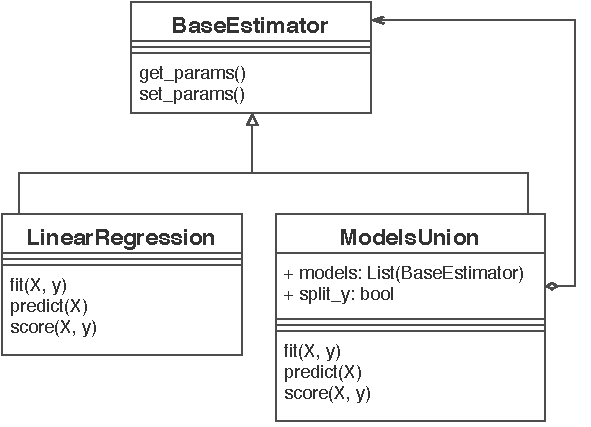
\includegraphics[width=10cm]{content/images/munion_class}
        \caption[Models-union class]{Class diagram of \textit{ModelsUnion}. Scikit-learn tends to use "duck typing", so building a model which supports require methods suffices for compatibility. Internal classes such as \textit{BaseEstimator} provide boilerplate code and is used for clarity and convenience intent.} 
        \label{fig:munion} 
    \end{figure}  

    ModelsUnion class puts the compositional model on one line with other surrogate models. It allows us uniformly validate many surrogate models and combine them in a surrogate portfolio.

% --------------------------------------------------------------------------------------------
% ---------------------------------------------------       Optimization orchestrator     
% --------------------------------------------------------------------------------------------
\section{Optimization orchestrator}
    The \textit{TutorModel} class is the orchestrator of all optimization's processes. It holds a surrogate portfolio, makes validation decisions, combines valid surrogate hypothesis and brings them together with optimization solvers (Figure \ref{fig:tutor_activity}).

    %! [ === Model product line === ]


    % ---------------------------------------------------        Validation
    \subsection{Surrogates validation}
        Each surrogate pass validation in several stages (Figure \ref{fig:simsim_activity_validation}): 1) Surrogate selection based on cross-validation results. In this stage define lower bound for overall accuracy. We notice that pass this threshold does not guarantee that surrogate is useful, but we sure that lower values detect models as useless. By default threshold \#1 defines as R2 less than 0.65. 2) Check accuracy in the region of interest. Finalist models chacks on unseen data to validate extrapolation quality and accuracy in optimal points. By default, R2 at this stage is also should be more than 0.65. Accuracy in optimal points is used for sorting champion models and corresponding solutions. Threshold's values selected from practical and theoretical use.

            % ==== activity_validation
            \begin{figure}
                \centering
                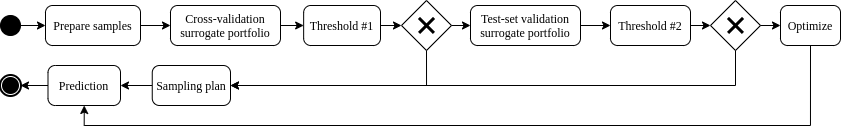
\includegraphics[width=\textwidth]{content/images/simsim_activity_workflow}
                \caption[General workflow activity]{General optimization workflow for model-based optimization iteration with validation in two stages.}
                \label{fig:simsim_activity_validation}
            \end{figure}

        The test set by default is 25\%. On left 75\% used cross-validation in 4 rounds. It means that gained four folds of samples and models training perform in three folds and testing on the fourth fold. It performs results for select or rejects surrogates combinations. After on test set gain information about the quality of possible solutions from surrogate 


    % ---------------------------------------------------        Portfolio        
    \subsection{Hypothesis portfolio}
    In general, surrogate models can be divided into two groups: a multi-output model for all objectives and compositional model with single-output models. All models pass validation equally, but after cross-validation single-objective models should combine in the complex surrogate hypothesis. 
    Ultimately, all objectives should be restored from valid surrogates and if some objective dimension has more models than other, last duplicate themselves to fill a gap. After complete restoring, compositional models with multi-output models validate further on the test set.

    % In the case of mixed surrogates models portfolio, validation pass in two groups: multi-objectives and single objective surrogates. In single-objective surrogates group must additionally restore complite hypotheisis for the multi-dimensional objective surface.

        % ==== Figure
        \begin{figure}
            \centering
            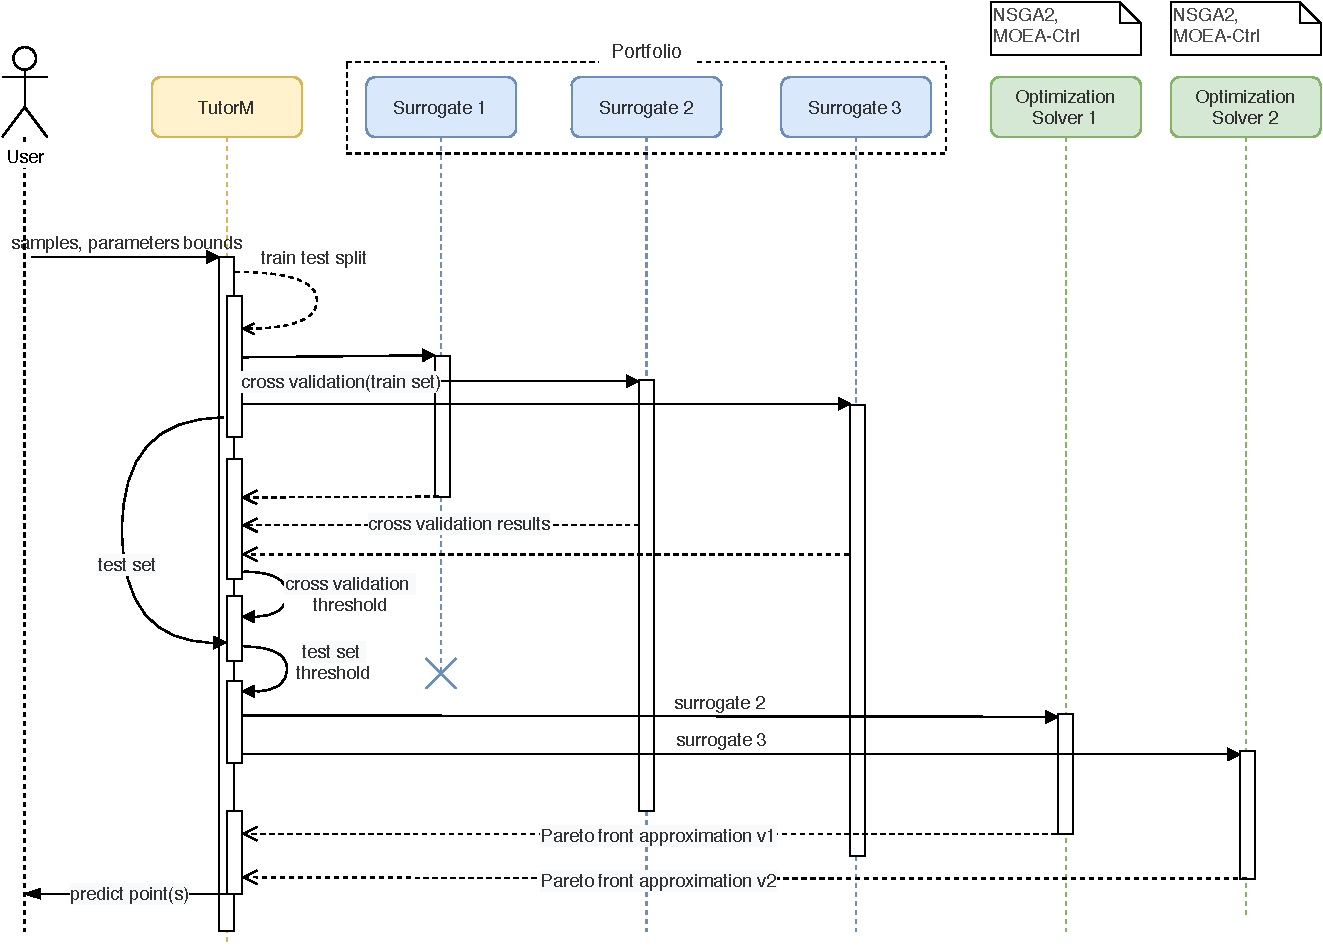
\includegraphics[width=\textwidth]{content/images/portfolio_validation_solv}
            \caption[Portfolio validation activity]{This is a validation and optimization workflow of several surrogates}
            \label{fig:tutor_activity}
        \end{figure}



    % ---------------------------------------------------        Sampling strategy
    \subsection{Sampling strategy} In many practical problems, only a restricted budget is spendable. Each evaluated point should be informative to reduce cost and improve interpolation by models. The most straightforward method of sampling design is a random witch for small sample sizes, that often produce clusters of samples. Conversely, there are also quasi-random distributions that produce informative samples that cover space more evenly. Most popular algoruthms are Sobol\cite{Sobol1999} and Latin hypercube sampling. 
    Out of the box, we provide Sobol sampling and random sampling.
    
    
    % Oversampling and undersampling in data analysis. Alleviate imbalance in the dataset. 
    % Imbalance in dataset is not always a problem, more so for optimization tasks. 

    % The main gain for models not to provide best accuracy on all search space but provide possible optimum regions.
    % Accuracy in prediction optimal regions or points from there will direct the search in the right direction.

    % Predictor variables can legitimately over- or under-sample. 
    % In this case, provided a carefully check that the model assumptions seem valid.

    % for other set of parameters, and make a choice from more diverse pool of models.

% --------------------------------------------------------------------------------------------
% ---------------------------------------------------       Solvers      
% --------------------------------------------------------------------------------------------
\section{Optimization solvers}


    Solvers role is to apply an optimization algorithm on the surrogate and find a solution(s). Most solvers implemented with Multi-objective evolutionary algorithms such as NSGA2, MOEA/D, Multi-objective Ant Colony Optimizer (MACO) or Nondominated Sorting Particle Swarm Optimizer (NSPSO). 
    Specifically added solver with a combination of several multi-objective genetic algorithms with a shared population (MOEA-Ctrl).

    Accordingly, on this step, a version of the solver with a scalarization of surrogates values possible witch optimize with any optimal heuristics. In this case, only one optimal point is obtained from the Pareto front, so the process must be repeated as many times as necessary to obtain the required count. 

    Optimization framework requires the definition of custom problems. Optimization algorithm receives the surrogate model as a parameter and builds custom optimization problem on it. In the case of a genetic algorithm, gain the perspective population of parameters, that could be selected as a Pareto front approximation. If several surrogates valid - several Pareto-front approximations obtain. There are two approaches to select the most informative solutions: 1) select Pareto approximation from surrogate with the highest accuracy in non-dominated points. 2) Assume that all approximations are valid and all points could be selected. In this case, intersection predictions from samples have a higher probability of being selected

    For singl-objective problem was adopted Extended Ant Colony Optimization algorithm (gaco). Feature of this algorithm consist in applying Gausian process regresion to generate future generations of ants. 

    All default solver allgorithms are implemanted in pygmo2 \cite{francesco_biscani_2019}.
    % Optimization algorithms. MOEA. A Python platform\cite{francesco_biscani_2019}  to perform parallel computations of optimisation tasks (global and local) via the asynchronous generalized island model.

    % decorators for single-objective solver with multi-objective surrogate 








% ----------    Designing a Sampling Plan
% \paragraph{Designing a Sampling Plan} The most straightforward way of sampling a design space in a uniform fashion is by \cite{EngSurMod} means of a rectangular grid of points. 
% Random sampling has the downside that for small sample sizes, there is often signficant clustering of samples, which is not ideal for interpolation since clustered samples can be wasteful. Instead, often a better option is to use a Latin hypercube, which enforces a condition that sample bins may not share the same coordinates for any coordinate axis







% Without automated tools, it can take days for experts to review just a few dozen examples.  In that same time, an automatic tool can explore thousands to millions to billions more solutions. People find it an overwhelming task just to certify the correctness of conclusions generated from so many results.


% Managing complex execution Strategies


% The simplifications are mean to discard the superfluous details that are unlikely to generalize to new instances. However, to decide what data to discard and what data to keep, you must make a hypothesis. For example, a linear model makes the hypothesis that the data is fundamentally linear and that the distance between the instances and the straight line is just noise, which can safely be ignored.



% sklearn 'duck typing'. This means that estimators are defined by interface, not by inheritance, where the interface is entirely implicit as far as the programming language is concerned.

% Variants in the evaluation of sets of solutions for each hypothesis. Each hypothesis has quality metrics. Solution(s) from each hypothesis have also own metrics.


% Intuition of why random forest is a good model: •Good at non-linearity, multi-modality and non-smoothness. A decision tree is a non-parametric supervised machine learning method widely used to formalize decision making processes across a variety of fields. The combination of many weak regressors (binary decisions) allows approximating highly non-linear and multi-modal functions with great accuracy. In addition, random forests naturally deal with categorical and ordinal variables which are important in computer systems optimization.


Workflow stages:
\begin{enumerate}
    \item Cross-Validation $\rightarrow$ Validation threshold
    \item Test-set score $\rightarrow$ Score threshold
    \item Surrogate models sort
    \item Optimization algorithm(s)
    \item MO infill criteria
\end{enumerate}

There are main approaches how produce single solution: 
\begin{itemize}
    \item Solution from best hypothesis. Sorting
    \item Bagging solution
    \item Voting solution                
\end{itemize}
